\documentclass[tikz,border=5pt]{standalone}
\usepackage{tikz}
\usetikzlibrary{positioning, shapes.geometric, arrows.meta, fit, backgrounds, calc, chains}

\begin{document}
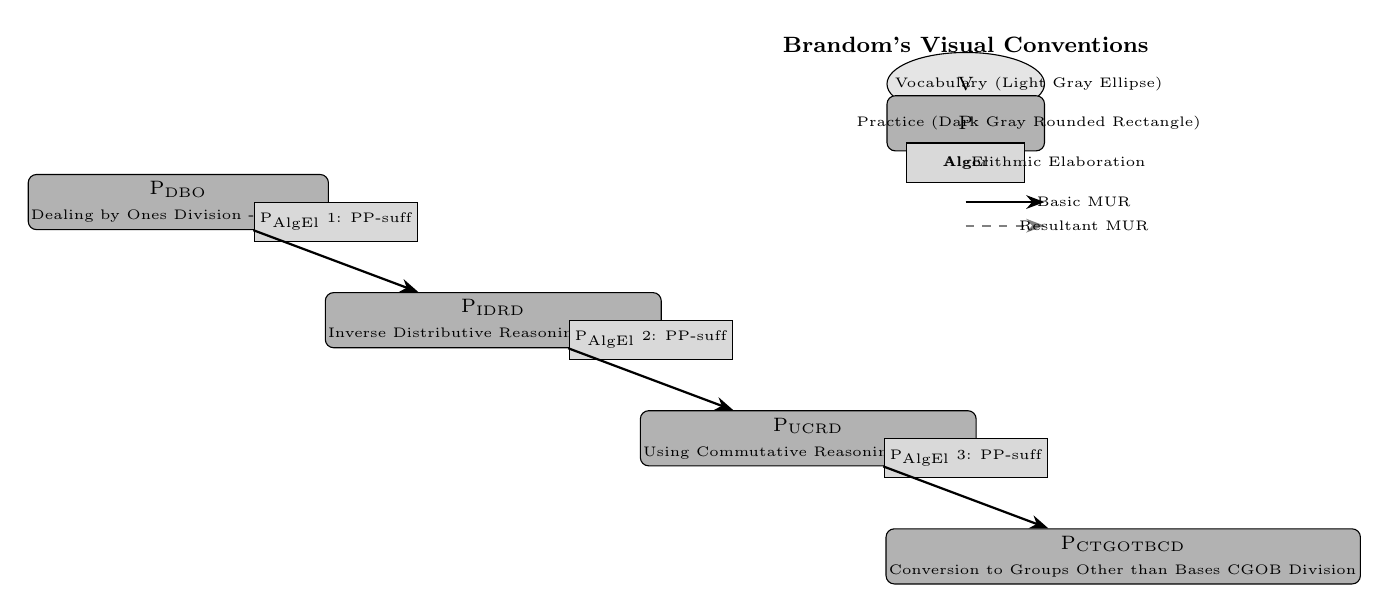
\begin{tikzpicture}[
  % Node Styles - Following Brandom's conventions exactly
  vnode/.style={ellipse, draw, fill=gray!20, text=black, minimum height=0.8cm, minimum width=2.0cm, align=center, font=\scriptsize},
  pnode/.style={rectangle, rounded corners=3pt, draw, fill=gray!60, text=black, minimum height=0.7cm, minimum width=2.0cm, align=center, font=\scriptsize, inner sep=1pt},
  % Arrow Styles
  solidarrow/.style={-Stealth, thick, black},
  dashedarrow/.style={dashed, -Stealth, thick, gray},
  % Special Elements
  algelelement/.style={rectangle, fill=gray!30, draw, inner sep=2pt, minimum width=1.5cm, minimum height=0.5cm, align=center, font=\tiny},
  textarrow/.style={align=center, inner sep=1pt, font=\tiny}
]

\node[pnode] (DBO) at (0,8.0) {P\textsubscript{DBO}\\\textsubscript{Dealing by Ones Division - Sharing}};
\node[pnode] (IDRD) at (4,6.5) {P\textsubscript{IDRD}\\\textsubscript{Inverse Distributive Reasoning Division}};
\node[pnode] (UCRD) at (8,5.0) {P\textsubscript{UCRD}\\\textsubscript{Using Commutative Reasoning Division}};
\node[pnode] (CTGOTBCD) at (12,3.5) {P\textsubscript{CTGOTBCD}\\\textsubscript{Conversion to Groups Other than Bases CGOB Division}};
\node[algelelement] (AlgEl_1) at (2.0,7.75) {P\textsubscript{AlgEl} 1: PP-suff};
\draw[solidarrow] (DBO) -- (IDRD);
\node[algelelement] (AlgEl_2) at (6.0,6.25) {P\textsubscript{AlgEl} 2: PP-suff};
\draw[solidarrow] (IDRD) -- (UCRD);
\node[algelelement] (AlgEl_3) at (10.0,4.75) {P\textsubscript{AlgEl} 3: PP-suff};
\draw[solidarrow] (UCRD) -- (CTGOTBCD);

% Legend
\node at (10,10) {\footnotesize\bfseries Brandom's Visual Conventions};
\node[vnode] at (10,9.5) {V};
\node at (10.8,9.5) {\tiny Vocabulary (Light Gray Ellipse)};
\node[pnode] at (10,9) {P};
\node at (10.8,9) {\tiny Practice (Dark Gray Rounded Rectangle)};
\node[algelelement] at (10,8.5) {AlgEl};
\node at (11,8.5) {\tiny Algorithmic Elaboration};

% Arrow legend
\draw[solidarrow] (10,8) -- (11,8);
\node at (11.5,8) {\tiny Basic MUR};
\draw[dashedarrow] (10,7.7) -- (11,7.7);
\node at (11.5,7.7) {\tiny Resultant MUR};

\end{tikzpicture}
\end{document}
